\documentclass[a4paper,12pt]{article}

\usepackage{rotating}
\usepackage[top=1in, bottom=1in, left=0.75in, right=0.75in]{geometry}
\usepackage{graphicx}
\usepackage[numbers,square,sort&compress]{natbib}
\usepackage{setspace}
\usepackage[cdot,mediumqspace,]{SIunits}
\usepackage{caption}
\usepackage{subcaption}
\usepackage{mathtools}
\usepackage{authblk}
\usepackage{float}
\renewcommand{\thesubsection}{\thesection.\alph{subsection}}
\providecommand{\e}[1]{\ensuremath{\times 10^{#1}}}

\begin{document}
\onehalfspacing
\title{PHY 407 Lab 7}
\author{Natalie Price-Jones, 999091021}
\date{24 October 2014}
\affil{\small{natalie.price.jones@mail.utoronto.ca}}
\maketitle

\section{Question 1}

For the implicit trapezoid method, we can derive the growth factor for ODE $dy/dt = \lambda y = f(y)$ starting from the expression for the $k + 1$th point in terms of the $k$th point.

\begin{eqnarray}
y_{k+1} &=& y_k + \frac{h_k}{2}[f(y_k) + f(y_{k+1})]\nonumber\\
y_{k+1} &=& y_k + \frac{h_k}{2}[\lambda y_k + \lambda y_{k+1}]\nonumber\\
\left(1 - \lambda \frac{h_k}{2}\right) y_{k+1} &=& \left(1 + \lambda\frac{h_k}{2}\right)\nonumber\\
y_{k+1} &=& \left[\frac{1 + \lambda\frac{h_k}{2}}{1 - \lambda\frac{h_k}{2}}\right]y_k\nonumber\\
y_{k+1} &=& \left[\frac{1 + \lambda\frac{h_k}{2}}{1 - \lambda\frac{h_k}{2}}\right]^k y_0\nonumber
\end{eqnarray}

Our stability constraint requires the absolute value of the growth factor to be less than one. In this case the growth factor is:

\begin{eqnarray}
\frac{1 + \lambda\frac{h_k}{2}}{1 - \lambda\frac{h_k}{2}}.\nonumber
\end{eqnarray}

This means our condition on stability is:

\begin{eqnarray}
\label{eqn:growth}
\left|\frac{1 + \lambda\frac{h_k}{2}}{1 - \lambda\frac{h_k}{2}}\right| \leq 1\\
\left|1 + \lambda\frac{h_k}{2}\right| \leq \left|1 - \lambda\frac{h_k}{2}\right|\nonumber
\end{eqnarray}

In terms of the two parameters $\lambda$ and $h_k$, we have shown that the solution is stable iff $\lambda h_k\leq 0$. However, since a zero step size is meaningless from a computational perspective and $\lambda = 0$ gives our ODE a trivial solution, we can logically restrict to stable solutions with $\lambda h_k < 0$. This means that we have the following set of conditions:

\begin{eqnarray}
&\mathrm{if}&\: \lambda < 0,\:\mathrm{then}\:h_k > 0\nonumber\\
&\mathrm{if}&\: h_k < 0,\:\mathrm{then}\:\lambda > 0\nonumber
\end{eqnarray}

%Regions of stability are shown in Figure \ref{fig:q1} below.

%\begin{figure}[H]
%\centering
%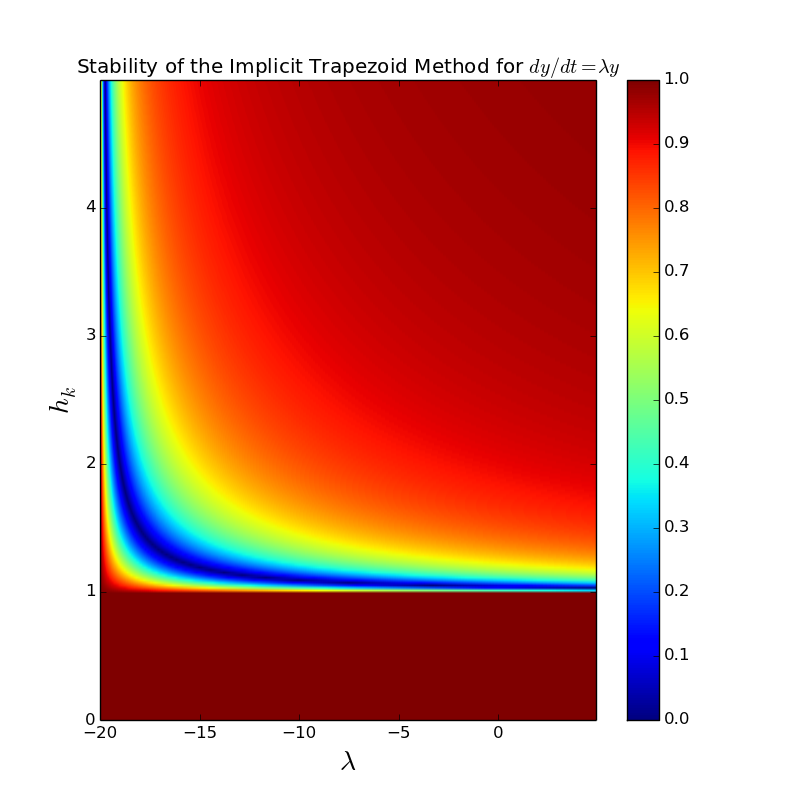
\includegraphics[width = \linewidth]{lab7q1.png}
%\caption{Value of the left hand side of Equation \ref{eqn:growth} for varying $\lambda$ and $h_k$ }
%\label{fig:q1}
%\end{figure}

The Taylor expansion of $y(t + h)$ is given by:

\begin{eqnarray}
y(t+h) &=& y(t) + hy'(t) + O(h^2) \nonumber\\
	   &=& y(t) + hf(y(t),t) + O(h^2)\nonumber\\
\implies y(t_{k+1}) &=& y(t_k) + h_k\lambda y(t_k) + O(h_k^2)\nonumber
\end{eqnarray}

Subtract this from the expression for $y_{k+1}$:

\begin{eqnarray}
y_{k+1} - y(t_{k+1}) = \left[\frac{1 + \lambda\frac{h_k}{2}}{1 - \lambda\frac{h_k}{2}}\right]y_k - (1+h_k\lambda)y(t_k) + O(h_k^2)\nonumber
\end{eqnarray}

If we attempt to find the local error $l$ by assuming no error prior to the $k+1$ step, we find:

\begin{eqnarray}
y_{k+1} - y(t_{k+1}) &=& \left[\frac{1 + \lambda\frac{h_k}{2}}{1 - \lambda\frac{h_k}{2}}\right]y_k - (1+h_k\lambda)y_k + O(h_k^2)\nonumber\\
y_{k+1} - y(t_{k+1}) &=& \left[\frac{1 + \lambda\frac{h_k}{2}}{1 - \lambda\frac{h_k}{2}} - (1+\lambda h_k)\right]y_k + O(h^2_k)\nonumber\\
y_{k+1} - y(t_{k+1}) &=& \left[\frac{1 + \lambda\frac{h_k}{2} - (1+\lambda h_k)(1-\lambda\frac{h_k}{2})}{1-\lambda\frac{h_k}{2}}\right]y_k + O(h_k^2)\nonumber\\
y_{k+1} - y(t_{k+1}) &=& \left[\frac{1 + \lambda\frac{h_k}{2} - 1 + \lambda^2\frac{h_k^2}{2} - \lambda h_k + \lambda\frac{h_k}{2}}{1-\lambda\frac{h_k}{2}}\right]y_k + O(h_k^2)\nonumber\\
y_{k+1} - y(t_{k+1}) &=& \left[ \frac{\lambda^2\frac{h_k^2}{2}}{1-\lambda\frac{h_k}{2}}\right]y_k + O(h_k^2)
\label{eqn:local}
\end{eqnarray}

Given that if $l = O(h_k^{p+1})$ then that accuracy is $p$, it should be possible to determine from Equation \ref{eqn:local} the accuract of the implicit trapezoid method, however I am not sure how to interpret my result.

\section{Question 2}

Comparing Figure \ref{fig:q2} and Figure \ref{fig:q2a} makes it obvious that integration with a fixed step size requires many more points of evaluation. As expected, in Figure \ref{fig:q2}, spacing between evaluation points becomes smaller in regions where the function changes quickly, and spreads out where the functions change slowly.

\begin{figure}[H]
\centering
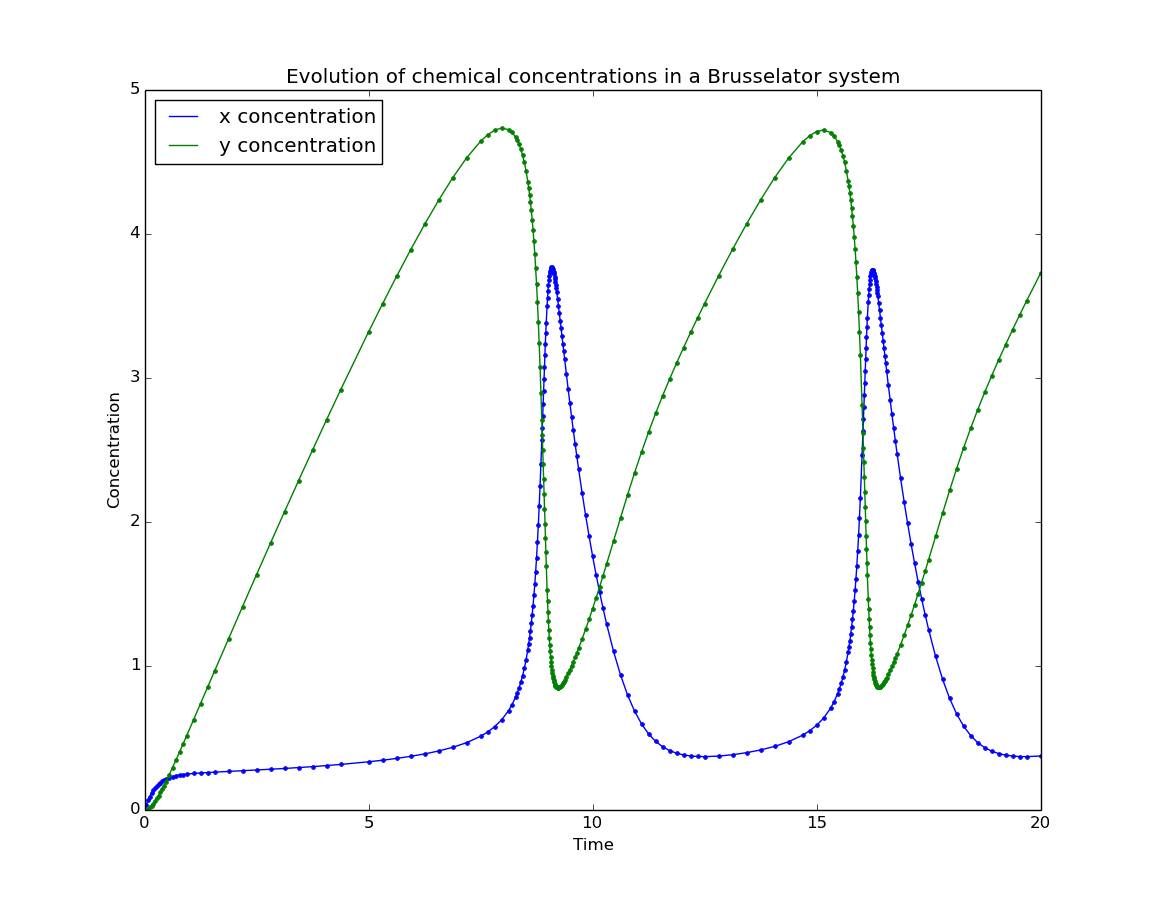
\includegraphics[width = \linewidth]{lab7q2.png}
\caption{Concentrations over time computed using an adaptive step size}
\label{fig:q2}
\end{figure}

\begin{figure}[H]
\centering
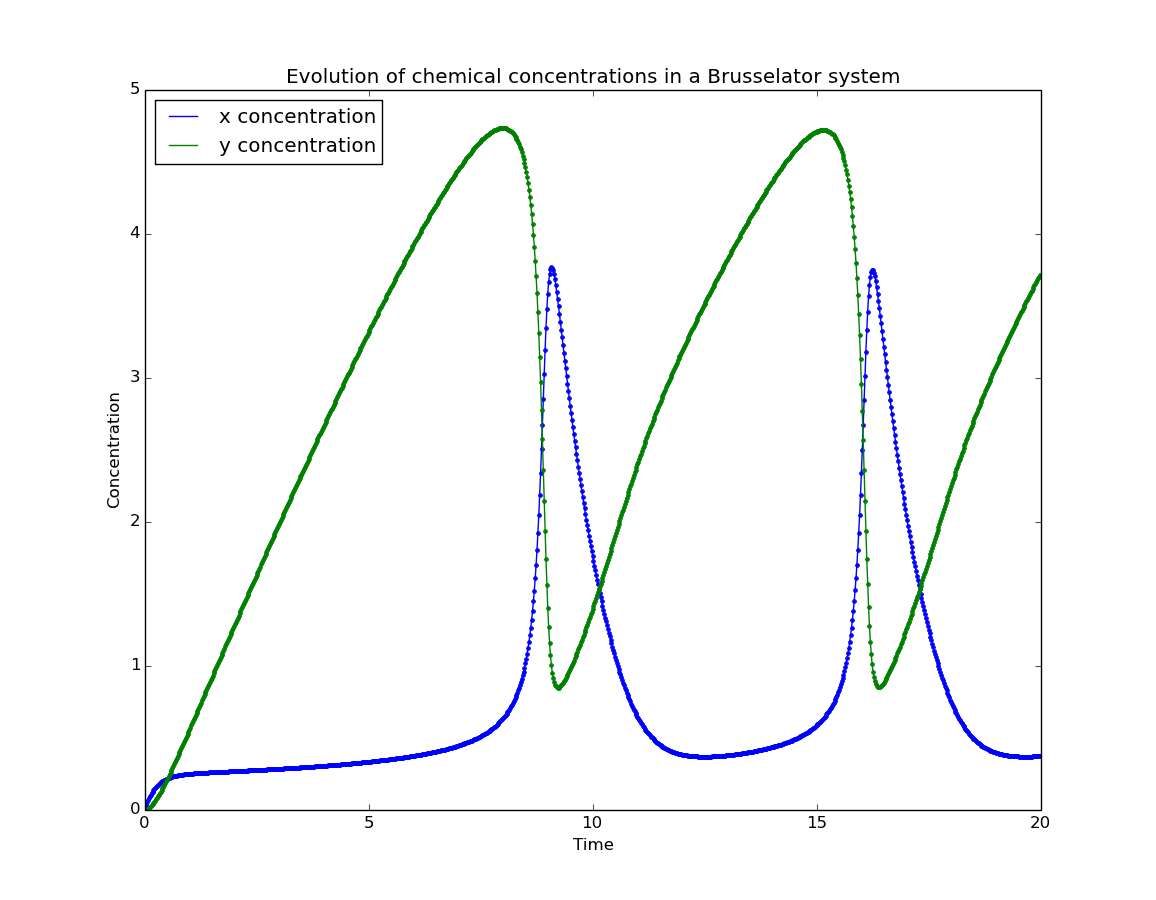
\includegraphics[width = \linewidth]{lab7q2additional.png}
\caption{Concentrations over time computed using an fixed step size}
\label{fig:q2a}
\end{figure}

\section{Question 3}

Denote the ground state with the index 0, and the $n$th excited with the index $n$. Then the energy eigenvalues of the harmonic potential Hamiltonian in a square box are as follows.

\begin{eqnarray}
E_0 &=& 138.024 \:\mathrm{eV}\nonumber\\
E_1 &=& 414.072 \:\mathrm{eV}\nonumber\\
E_2 &=& 690.120 \:\mathrm{eV}\nonumber
\end{eqnarray}

The difference between pairs of sequential values is $276.048$ eV, so the the energy eigenvalues are equally spaced, as expected.

\section{Question 4}

Denote the ground state with the index 0, and the $n$th excited with the index $n$. Then the energy eigenvalues of the anharmonic potential Hamiltonian in a square box are as follows.

\begin{eqnarray}
E_0 &=& 205.307 \:\mathrm{eV}\nonumber\\
E_1 &=& 735.691 \:\mathrm{eV}\nonumber\\
E_2 &=& 1443.569 \:\mathrm{eV}\nonumber
\end{eqnarray}

\section{Question 5}

\begin{figure}[H]
\centering
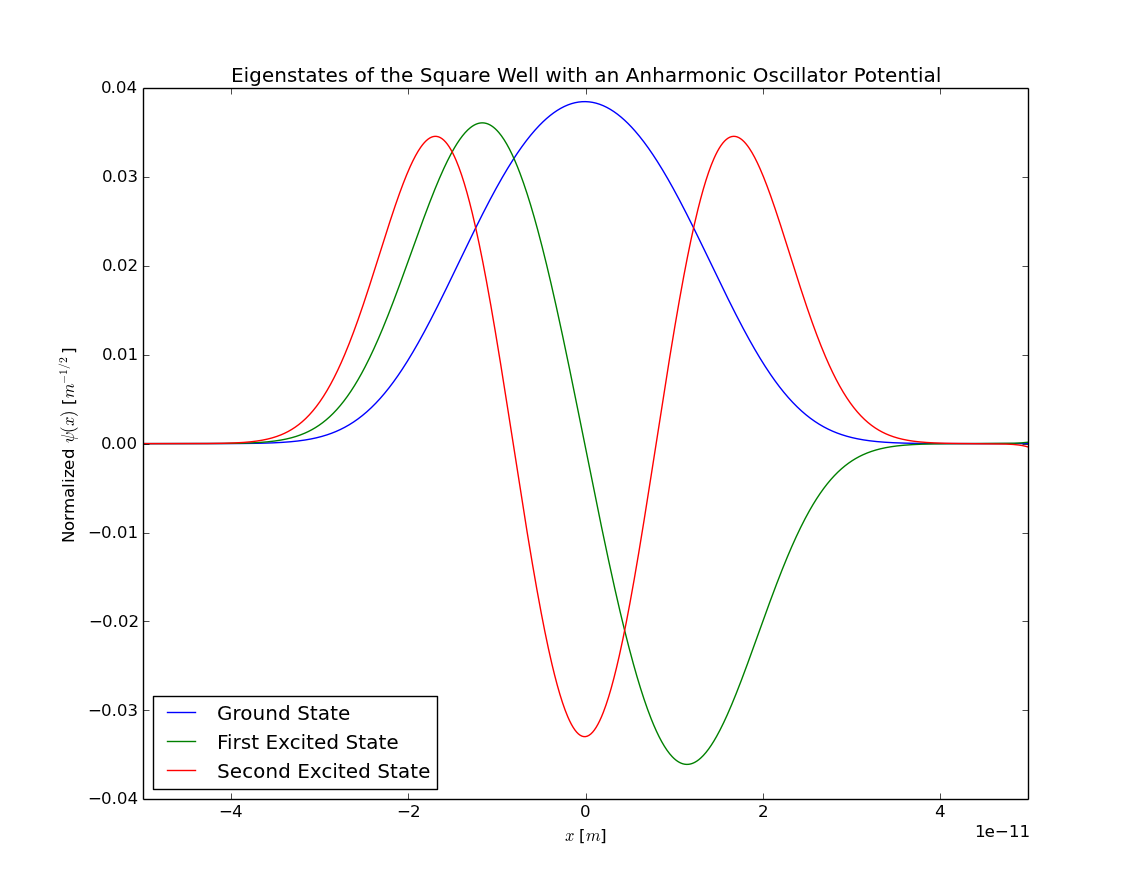
\includegraphics[width = \linewidth]{lab7q5.png}
\caption{}
\label{fig:q5}
\end{figure}

\end{document}





